\chapter{Methodology}

\section{Graphs}
As mentioned in the previous chapter, graphs are good analytical tools when studying complex systems. Since we will use graphs extensively throughout this thesis, it is important to establish an understanding of basic graph properties. Figure \ref{fig:generalGraph} depicts the basics of an unweighted graph, where the edges are not assigned any value. Weighted edges can be useful to e.g. reflect capacity constraints such as a link's maximum bandwidth, or the length of a road (edge), but will not be used in this thesis. Other common definitions used when describing graphs are listed below \cite{audestad}:
\begin{itemize}
\item Edge degree: Number of edges connected with a node.
\item Hub: Node with high edge degree.
\item Cycle: A chain originating and terminating at the same node.
\item Cluster: Subgraph of highly connected nodes.
\item Cluster coefficient: Probability for two nodes to be adjacent to a third node.
\item Clique: Subgraph where all nodes are adjacent (cluster coefficient = 1).
\item Small world graph: Graph with small diameter and large cluster coefficient (e.g. the Internet and A-B graphs, described in section \ref{ABgraph}).
\end{itemize}

\begin{figure}[h]
\centering
\begin{tabular}{@{}c@{}}
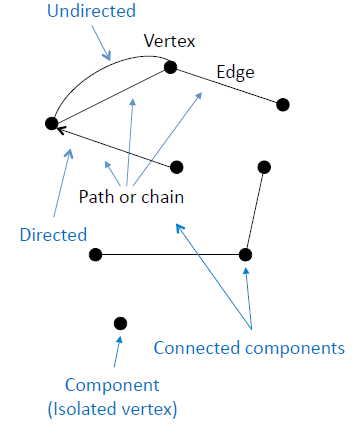
\includegraphics[width=0.4\textwidth]{../Figures/generalGraph.png}
\end{tabular}
\caption{\label{fig:generalGraph} General graph \cite{audestad}.}
\end{figure}

\section{Random Graphs}
Cyber-insurance covers many fields, from financial transactions and software development to computer networks. Many of these fields share a common characteristic, they can all be described as a graph, and often as a random graph. Therefore, the study of random graphs is of special concern. The research on random graphs is fairly new compared to other mathematical discoveries. The first extensive results where found by Erdös and Rényi in 1959, hence the resulting structures were called  E-R graphs. Later and probably with more accurate results were the work of Albert-Barabási in 1999 \cite{audestad}, leading to the characterization of A-B graphs. 
\subparagraph{Erdös-Rényi Graphs.}
E-R graphs are networks created between a fixed number of $n$-nodes, where each node connects to another of the $n-1$ nodes with 
probability $p$. The resulting graph will on average contain $\frac{n(n-1)p}{2} \approx \frac{n^{2}p}{2}$ edges \cite{barabasi}. 
By analysing the graph, the authors found some interesting properties:

\begin{itemize}
\item If $p<n^{-2}$  then there is no edges in the graph. 
\item If $p=c/n$ where c is a constant between $1 < c < log\: n$, the graph will provoke a single large component to grow within the graph.
\item If $p>(ln\: n)/n$ then the graph is completely connected. 
\item If $p = 1/n$ triangles start forming in the graph. 
\end{itemize}

A fully connected E-R graph will have a short diameter similar to the Internet, and thus could be a very good description of structures similar to the Internet. However, the edge degree follows a Poisson distribution, which means that the edge degrees are peaking around the average value \cite{audestad}. E-R graphs do not capture the immense clustering coefficient which is present in networks such as the Internet. In other words, E-R graphs are not small world graphs, and a different graph structure is needed to model computer networks.
An interesting fact about these graphs is their vulnerability. These graphs are very vulnerable against random attacks, such as nature disasters, but robust against directed attacks. Due to the fact that if you remove all edges from one node, little damage is done, since the network is not dependent on only a few nodes. Every node has approximately the same node degree, and it is the sum of all the nodes' connections that creates the network.

\subparagraph{\label{ABgraph}Albert-Barabási Graphs.}
The structure which is believed to be most accurate for modelling computer networks are A-B graphs. A-B graphs are different from E-R graphs since they are scale-free, meaning that the vertices do not have a constant value throughout the entire graph. Albert and Barabási found that the edge degree of each vertex follows a power law distribution; meaning that the probability that the edge degree is $g$ is proportional to $g^{-\gamma}$
where $\gamma$ is usually a number between 2 and 3. This distribution is called a thick-tail distribution, because there is a significant probability that a node may have a very high degree \cite{audestad}.
These graphs are in contrast to E-R-graphs, very vulnerable to directed attacks, because if you take out a hub, mayor parts of the network will be affected. But the graph is very robust against random attacks, which is why most of the networks we observe in nature can be depicted as A-B-graphs.
A-B graphs can grow and become scale-free if every new node is connected to one or more already existing node with a probability proportional to the edge degree of that node. The paper present an algorithm that creates A-B graphs and Figure \ref{fig:ABgraphcreation} shows a graph that evolves from this algorithm:

\begin{itemize}
\item A new single vertex is added to the graph.
\item This vertex is connected to exactly two other vertices in the graph.
\item The probability that the new vertex connects to another vertex is dependent on the edge degree of the other vertex, higher edge degree meaning higher probability
\item There is only one edge between two vertices.
\end{itemize}


\begin{figure}[h]
\centering
\begin{tabular}{@{}c@{}}
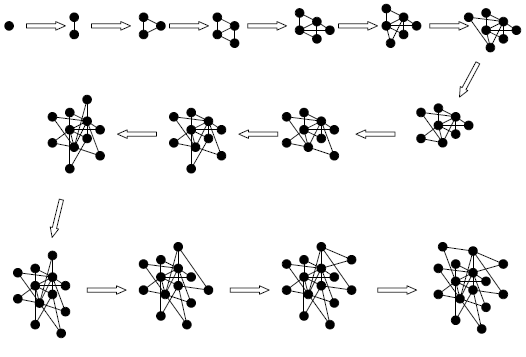
\includegraphics[width=0.8\textwidth]{../Figures/ABgraphcreation.png}
\end{tabular}
\caption{\label{fig:ABgraphcreation} Forming an A-B graph in 15 generations \cite{audestad}.}
\end{figure}

In addition to the high clustering coefficient Albert-Barabási showed that A-B-graphs have a fairly small diameter,
 which can be seen in Figure \ref{fig:ABgraphcreation}. 
The World Wide Web, neural networks, scientific referencing, co-authorship and many other types of networks are very similar to A-B graphs \cite{audestad}.

\section{Game Theory}
Here we will present some of the game theory concepts used in our models, for more thorough explanation of game theory, see: \cite{nisan2007algorithmic, watson2008strategy}.
\subparagraph{One shot game.}
This type of game assumes that players act at the same time instantly, therefore there is no causality. A game in strategic (normal) form can be described by three elements:
\begin{itemize}
\item the set of players $i \in I$, which we take to be the finite set ${1,2,....,I}$.
\item the pure-strategy space $s_{i}\in S_{i}$ for each player i, where $s_{i}$ is a possible action of player i.
\item and payoff functions $U$, which give the players utility functions for each profile $s=(s_{1},s_{2},...,s_{I})$ of strategies.
\end{itemize}
A general solution concept for games of economic interest is the Nash Equilibrium solution. A Nash Equilibrium is a profile of strategies such that each players strategy is a best response to the other player's strategies. 
\subparagraph{Nash Equilibrium.}
A pure strategy profile $s^{*}$ is a Nash equilibrium if, for all players $i$
\begin{equation}
U_{i}(s^{*}_{i},s_{-i}^{*})\geq U_{i}(s_{i},s^{*}_{-i}) \in S_{i}
\end{equation}

\subparagraph{Subgame-perfect equilibrium.}
A strategy profile $s$ is a subgame perfect equilibrium if it represents a Nash Equilibrium of every subgame of the original game.
\subparagraph{Socially optimal.}
A socially optimal outcome is the set of choices that maximizes the sum of all players' payoffs. 
\subparagraph{Price of Anarchy.}
The price of Anarchy (PoA) of a network game, measures the efficiency of the network, by comparing the equilibrium outcome with the socially optimal outcome. The reason for this possible inefficiency is that agents act selfishly and do not necessarily consider other agents' payoff when choosing an action. In our thesis, the price of anarchy will be a number between 0 and 1, where 1 is the socially optimal outcome.
\subparagraph{Stackelberg game.}
Also known as a leader-follower game, it introduces multiple stages. The leader commits himself first, chooses his strategy, then the followers respond sequentially. The Stackelberg model can be solved to find the subgame perfect Nash Equilibrium, i.e. the strategy profile that serves each player best, given the strategies of the other players and that entails every player playing in a Nash Equilibrium in every subgame.
\subparagraph{Bayesian game.}
In Bayesian games, information about the other players' characteristics is incomplete. In these types of games, there is one player(the agent) who knows both types, and another player (the principal) who does not know the type of the other player. There are two types of equilibriums in this game:
A pooling equilibrium, is an equilibrium where both types of the agent choose the same action, i.e. the principal is not able to distinguish the two types. 
A separating equilibrium is an equilibrium where the agents of different types choose different actions, and thus the principal is able to determine the agent's type by observing his actions.
\subparagraph{Pairwise stability.}
A graph is pairwise stable if:
 \begin{enumerate}
\item \textit{No node wishes to delete a link he is involved in.}
\item \textit{If there exists a node which wants to add a link, then the node at the other end of the link does not want to establish this link.}
\end{enumerate} 
Pairwise stable networks are robust to one-link deviations, where link
severance is unilateral, while link creation is bilateral and under mutual consent of the two involved
players \cite{calvo2009pairwise}.

\section{Netlogo}
In addition to analyzing the different models with game theory, we created a simulator for the models, in a program called Netlogo. Netlogo is a programmable modeling environment for simulating natural and social phenomena. It is well suited for modeling complex systems developing over time \cite{netlogo}.
Netlogo is well suited to model our complex network formation games, and at the same time Netlogo provided us with a good graphical user interface that enabled us to see the result of the games, and also to easily adjust the different parameters. It was especially of use when facing models that were difficult to analyze, because it gave us a good graphical result, showing how the network evolved, and the final resulting network.  
In Figure \ref{fig:netlogo} we see the user interface, which is used to set up the parameters, start the modeling, and showing the resulting network formation. Figure \ref{fig:netlogo-code} shows how the coding interface looked like. For detailed overview of the code used in our different models, see appendix.
\begin{figure}[h]
\centering
  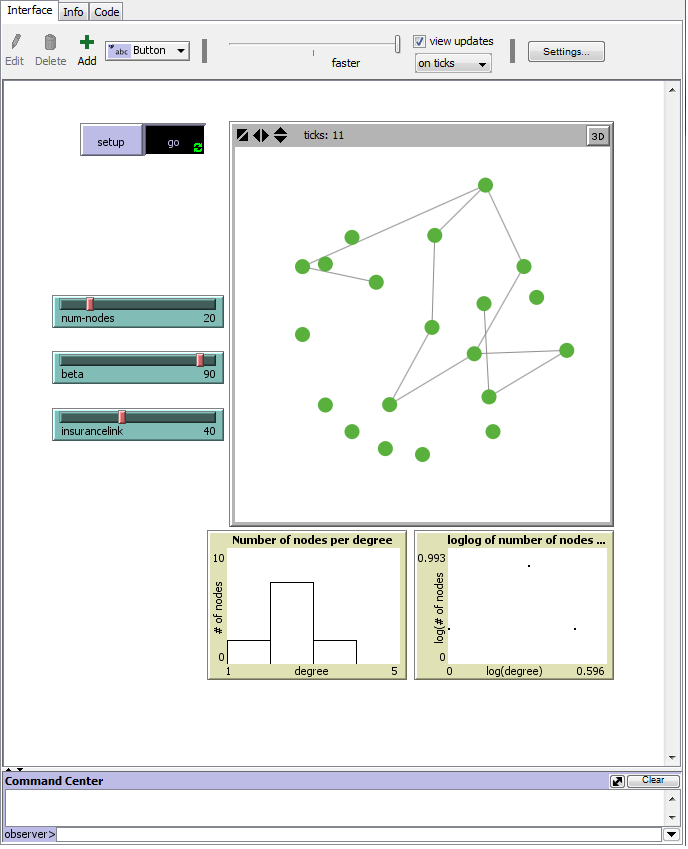
\includegraphics[width=0.9\linewidth]{../Figures/netlogoexample.png}
  \caption{\label{fig:netlogo} The figure shows a screen capture of Netlogo, while we are running one of our simulations.}

\end{figure}
\begin{figure}[h]
\centering
  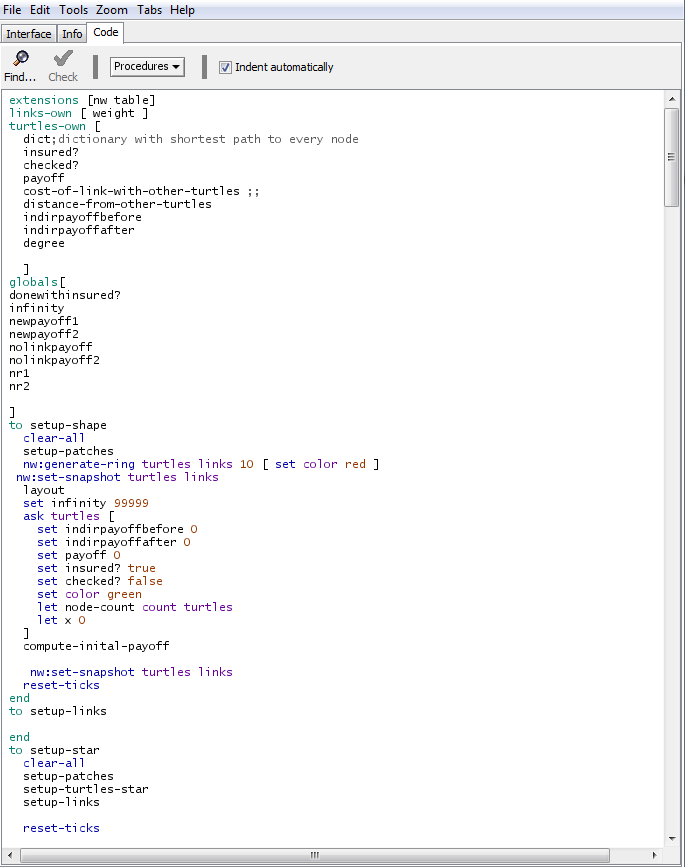
\includegraphics[width=0.9\linewidth]{../Figures/netlogocodeexample.png}
  \caption{\label{fig:netlogo-code} The figure shows how the code interface in netlogo looks like.}

\end{figure}



